%%%%%%%%%%%%%%%%%%%%%%%%%%%%%%%%%%%%%%%%%%%%%%%%%%%%%%%%%%%%%%%%%%%%%%%%%%%%%%%%
%2345678901234567890123456789012345678901234567890123456789012345678901234567890
%        1         2         3         4         5         6         7         8

\documentclass[letterpaper, 9 pt, conference]{ieeeconf}  % Comment this line out if you need a4paper

%\documentclass[a4paper, 11pt, conference]{ieeeconf}      % Use this line for a4 paper

\IEEEoverridecommandlockouts                              % This command is only needed if 
                                                          % you want to use the \thanks command

\overrideIEEEmargins                                      % Needed to meet printer requirements.

% See the \addtolength command later in the file to balance the column lengths
% on the last page of the document

% The following packages can be found on http:\\www.ctan.org
%\usepackage{graphics} % for pdf, bitmapped graphics files
%\usepackage{epsfig} % for postscript graphics files
%\usepackage{mathptmx} % assumes new font selection scheme installed
%\usepackage{times} % assumes new font selection scheme installed
%\usepackage{amsmath} % assumes amsmath package installed
%\usepackage{amssymb}  % assumes amsmath package installed
\usepackage{graphicx}
\usepackage{hyperref}
\usepackage{verbatim}
\title{\LARGE \bf
Exploration and Mapping with a Particle Swarm Controlled by Uniform Inputs on a Magnetic Setup
}


\author{Daniel Bao, Arun Mahadev, Aaron T. Becker% <-this % stops a space
\thanks{D. Bao, A.~Mahadev, and A.~Becker are with the Department of Electrical and Computer Engineering,  University of Houston, Houston, TX 77204-4005 USA 
      \protect\url{ aviswanathanmahadev@uh.edu,atbecker@uh.edu }}
\thanks{*This work was supported by the National Science Foundation under Grant No.\ \href{http://nsf.gov/awardsearch/showAward?AWD_ID=1553063}{ [IIS-1553063]} and \href{http://nsf.gov/awardsearch/showAward?AWD_ID=1619278}{[IIS-1619278]}.}% <-this % stops a space
}
\begin{document}



\maketitle
\thispagestyle{empty}
\pagestyle{empty}


%%%%%%%%%%%%%%%%%%%%%%%%%%%%%%%%%%%%%%%%%%%%%%%%%%%%%%%%%%%%%%%%%%%%%%%%%%%%%%%%
\section{Introduction}\label{sec:Introduction}
	This research deals with mapping a work space using a swarm of non-intelligent robots. Much work has been done in single robot mapping, but there is a gap of research for multiple robots exploring an environment using the same input commands, also known as global uniform control. In our previous work\cite{AAM}, we developed a ClosestFrontier algorithm, with frontiers being unknown boundary cells, that maps a discrete 2D work space using global uniform control. Here we expand its scope to 3D environments and implement a physical hardware setup using four orthogonal magnetic coils.
\section{Methods and Results}\label{sec:Methods and Results}
	For the physical setup, we use resin-bound acrylic to create a transparent work space compatible with the black paramagnetic particles suspended on the water's surface and a camera recording from below. This allows for more dynamic interactions as well as continuous boundaries. New challenges like wall friction, surface tension, and  hydrophobic interactions between the particles now arise from the physicality of the setup. These physical properties prove hardest to overcome in small branched maps because of the high meniscus and local minimum of water that the particles face . To address this problem, we designed our work spaces with optimized channel width and curved edges to avoid local minimums.
	
	Expanding the previous 2D simulation to 3D required us to increase the matrix dimensions and the nodes required to search with the ClosestFrontier algorithm but the extra dimension didn't require more moves to completely map the workspace when the free space count was the same. More simply, there is no trade off between dimensions and completeness of the explored work space. Only the complexity of the map matters, which means that for the same number of free spaces on a 2D and 3D map, the map with the more complex shape will require more total moves to map with the ClosestFrontier algorithm from previous work. Complex shapes are highly branched and take many turns and loops which makes mapping more time and process consuming. Examples are shown in Fig. 1 and 2.
\section{Discussion}\label{sec:Discussion}
	This research allows for precise control over weaker para-magnetic particles as well as a theoretical understanding of algorithmic efficiency in real world work spaces. Ultimately, medicinal applications in active targeted drug delivery and mapping vasculature as an alternative to traditional contrast agents are fields that can benefit from this research as well as more studies on non-invasive particle treatments. 
\begin{figure}
	%\vspace{30pt}
\begin{comment}
	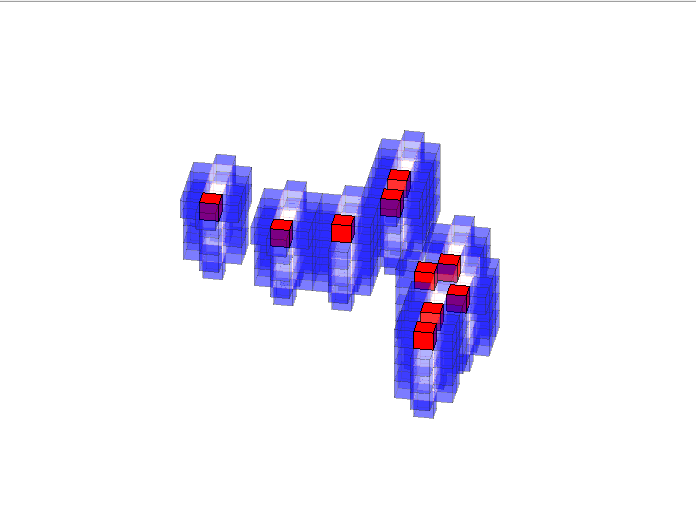
\includegraphics[height=0.2\paperheight]{3d1.png}
	\caption{The 3D simulation is shown above with red blocks being the particles, blue being the frontier cells, and white being free explored cells.}
\end{comment}
	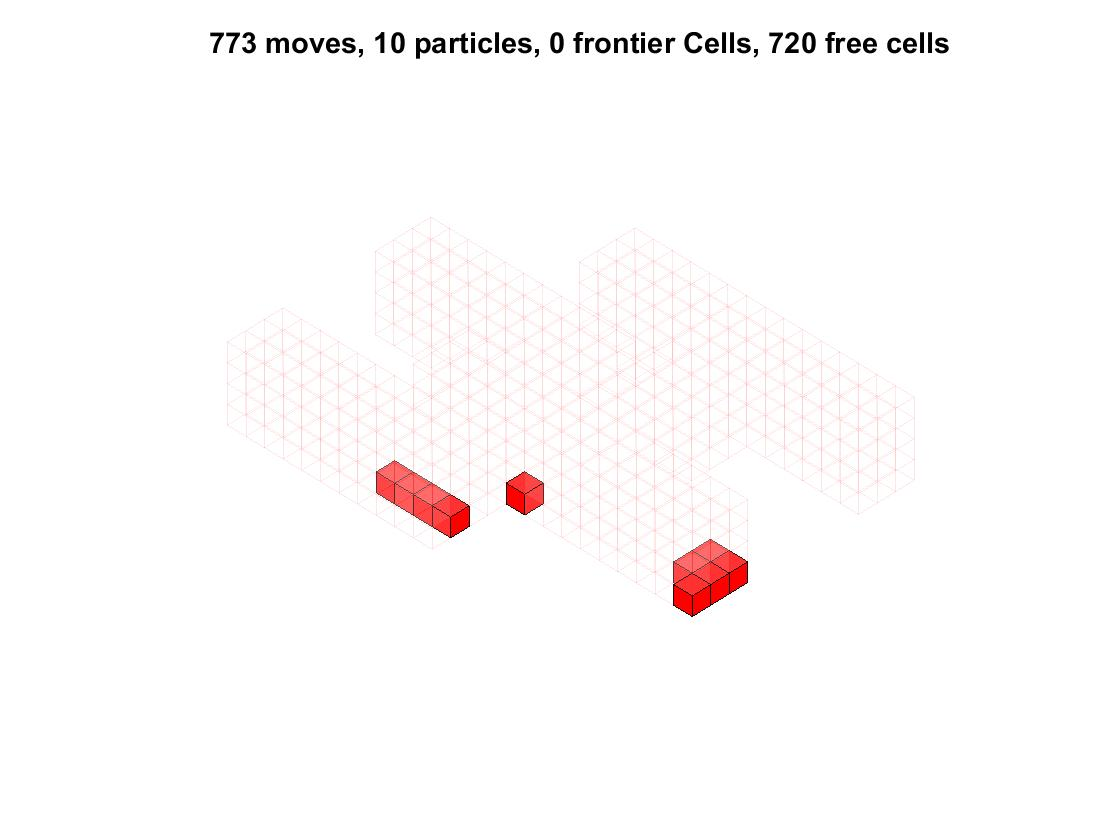
\includegraphics[height=0.2\paperheight]{10particles_3D.jpg}
	\caption{Here are 10 particles that have completely explored the same work space shown in Fig. 1. As shown, the work space is the University of Houston's initials with four layers. The white blocks are the mapped free spaces and everything else is an obstacle.}
	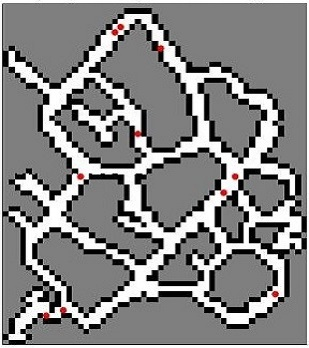
\includegraphics[height=0.2\paperheight]{10particles_final.jpg}
	\caption{For an equivalent number of free cells in 2D, more moves were required by the ClosestFrontier Algorithm due to the increased complexity of this vascular system based off of a leaf tissue sample. The black blocks are the mapped obstacles, white blocks are the free spaces, and red blocks are the particles again.}
\end{figure}
\bibliographystyle{IEEEtran}
\bibliography{abstract}

\end{document}
